% Technical report. Every result number is a macro from numbers.tex, generated by tools/p4_numbers.py from committed results;
% tests/test_p4_numbers.py checks the table and that no result-like decimal is typed into this file by hand.
% Text licensed CC BY 4.0 (see paper/README.md); code in this repository is Apache-2.0.
% Version 1.1 adds P2.8, P5 and P6 (docs/p4-plan.md, amendment 1).
\documentclass[11pt,a4paper]{article}
\usepackage[margin=2.5cm]{geometry}
\usepackage{amsmath,amssymb}
\usepackage{booktabs}
\usepackage{graphicx}
\usepackage[hidelinks]{hyperref}
\emergencystretch=3em

% Generated by tools/p4_numbers.py from committed result files. Do not edit by hand.

\newcommand{\PzeroKingstonHardware}{0.788}
\newcommand{\PzeroKingstonTheory}{0.945}
\newcommand{\PzeroFiveKingstonRaw}{0.786}
\newcommand{\PzeroFiveKingstonCorrected}{0.808}
\newcommand{\PzeroFiveGainMinPP}{1.5}
\newcommand{\PzeroFiveGainMaxPP}{3.3}
\newcommand{\PoneOptimumTruth}{82.2\%}
\newcommand{\PoneGateInstances}{588}
\newcommand{\PoneGatePassed}{588}
\newcommand{\PoneSafeOverCritThree}{47}
\newcommand{\PoneSafeOverCritFour}{106}
\newcommand{\PoneSAOracle}{0.641}
\newcommand{\PoneSAMaxAbs}{0.355}
\newcommand{\PoneSASafe}{0.190}
\newcommand{\PoneQAOAMaxAbsThree}{0.077}
\newcommand{\PoneQAOAOracleThree}{0.029}
\newcommand{\PoneQAOAMaxAbsTwo}{0.578}
\newcommand{\PoneCZThreePthree}{238}
\newcommand{\PoneFiveTwoPoneCZ}{11}
\newcommand{\PoneFiveTwoPoneSim}{0.2140}
\newcommand{\PoneFiveTwoPoneHw}{0.1962}
\newcommand{\PoneFiveTwoPoneKept}{91.7\%}
\newcommand{\PoneFiveTwoPtwoCZ}{22}
\newcommand{\PoneFiveTwoPtwoSim}{0.5445}
\newcommand{\PoneFiveTwoPtwoHw}{0.4847}
\newcommand{\PoneFiveTwoPtwoKept}{89.0\%}
\newcommand{\PoneFiveThreePoneCZ}{58}
\newcommand{\PoneFiveThreePoneSim}{0.0201}
\newcommand{\PoneFiveThreePoneHw}{0.0180}
\newcommand{\PoneFiveThreePoneKept}{89.7\%}
\newcommand{\PtwoGateRejectedPct}{0.98}
\newcommand{\PtwoGateTruePairs}{38,683}
\newcommand{\PtwoILPGate}{888}
\newcommand{\PtwoHfourShare}{27.4\%}
\newcommand{\PtwoHfourLow}{23.7\%}
\newcommand{\PtwoHfourHigh}{31.5\%}
\newcommand{\PtwoFactorDefault}{0.303}
\newcommand{\PtwoFactorPure}{0.737}
\newcommand{\PtwoFactorBearing}{0.833}
\newcommand{\PtwoFactorBearingNoClutter}{0.933}
\newcommand{\PtwoQUBOGate}{517}
\newcommand{\PtwoQUBOGatePassed}{517}
\newcommand{\PtwoLRLowClutter}{99.5\%}
\newcommand{\PtwoGapClutterZero}{0.065}
\newcommand{\PtwoGapClutterTwo}{0.080}
\newcommand{\PtwoGapSpacingClose}{0.130}
\newcommand{\PtwoGapSpacingFar}{0.085}
\newcommand{\PtwoBenchInstances}{1,620}
\newcommand{\PtwoBenchInfeasible}{14}
\newcommand{\PtwoBenchGap}{43}
\newcommand{\PtwoBenchLR}{98.7\%}
\newcommand{\PtwoBenchSA}{63.3\%}
\newcommand{\PtwoBenchGreedy}{52.7\%}
\newcommand{\PtwoBenchGreedyNorm}{41.5\%}
\newcommand{\PtwoHthreeMaxAbs}{0.0687}
\newcommand{\PtwoHthreeOracle}{0.0304}
\newcommand{\PtwoGoRatio}{12.7}
\newcommand{\PtwoGoCZ}{29}
\newcommand{\PtwoSixAKept}{89.2\%}
\newcommand{\PtwoSixAHw}{0.4856}
\newcommand{\PtwoSixBSim}{0.0164}
\newcommand{\PtwoSixBHw}{0.0173}
\newcommand{\PtwoSixBGuess}{15.7}
\newcommand{\PtwoSixUsage}{18}
\newcommand{\PthreeOptimum}{-92.35}
\newcommand{\PthreeOptimumPaperEq}{-32.85}
\newcommand{\PthreeOptimumLarge}{-131.98}
\newcommand{\PthreeQualityA}{0.836}
\newcommand{\PthreePoptA}{0.0020}
\newcommand{\PthreeReversedA}{0.430}
\newcommand{\PthreeQualityC}{0.575}
\newcommand{\PthreeQualityD}{0.820}
\newcommand{\PthreeRandomMean}{0.582}
\newcommand{\PthreeRandomPninetyfive}{0.866}
\newcommand{\PthreeRandomAboveHeadline}{43.4\%}
\newcommand{\PthreeRandomBestOfAll}{0.995}
\newcommand{\PthreeLargeQualityPone}{0.534}
\newcommand{\PthreeLargeQualityPtwo}{0.759}
\newcommand{\PthreeLargeRandomMean}{0.150}
\newcommand{\PthreeLargeRandomAbove}{44.0\%}
\newcommand{\PtwoQUBOInfeasible}{17}
\newcommand{\PtwoHthreePurePositive}{96.7\%}
\newcommand{\PtwoHthreeSparsePositive}{33.3\%}
\newcommand{\PtwoPureCZ}{85}
\newcommand{\PtwoBenchLRInvalid}{16}
\newcommand{\PtwoBenchGreedyInvalid}{21}
\newcommand{\PtwoBenchLRGap}{88.4\%}
\newcommand{\PtwoSixBCZMin}{8}
\newcommand{\PtwoSixBCZMax}{57}
\newcommand{\PthreePaperHungarian}{-92.4}
\newcommand{\PthreeCOneDiff}{0.045}
\newcommand{\PthreeLargePaperOptimum}{-132.0}
\newcommand{\PthreeLargePaperPone}{20.4\%}
\newcommand{\PthreeLargePaperPtwo}{11.5\%}

% Constants that exist only in the research log (not machine-checkable):
\newcommand{\QPUSecondsPzero}{9}  % research log, P0 hardware sweep: IBM dashboard reading
\newcommand{\QPUSecondsTotal}{81}  % research log, P2.6: 63 s from dashboard readings plus 18 s reported by the P2.6 jobs

% Numbers reported by the paper under study (quoted, not results of this project):
\newcommand{\PthreePaperHeadline}{64.1}  % quoted from arXiv:2603.00785, Sec. 8.6 and Table 15 (percent of optimum)
\newcommand{\PthreePaperHeadlineSD}{3.3}  % quoted from arXiv:2603.00785, Sec. 8.6 (percentage points, three runs)
\newcommand{\PthreePaperTwoQubitGates}{433--435}  % quoted from arXiv:2603.00785, Sec. 8.6 and Table 4 (p = 3)
\newcommand{\PthreePaperSimPthree}{90.9}  % quoted from arXiv:2603.00785, Sec. 8.6 (simulator quality, p = 3, percent)

\graphicspath{{figures/}}

\title{Pre-registered small-scale experiments on quantum optimisation for multi-target data association and planning:
exact baselines, a reproducible benchmark, IBM hardware runs and two reproduction studies}
\author{Kiettisak Suthsilp\\
Independent researcher\\
ORCID \href{https://orcid.org/0009-0003-3249-990X}{0009-0003-3249-990X}\\
\texttt{kiettisak.suthsilp@gmail.com}}
\date{15 September 2026 --- version 1.1}

\begin{document}
\maketitle

\begin{abstract}
Data association --- deciding which measurement belongs to which target --- can be written as a quadratic unconstrained binary
optimisation (QUBO) problem and attacked with quantum annealing or the quantum approximate optimisation algorithm (QAOA).
Published results at this intersection are small and hard to check. This report collects five pre-registered studies in which every
hypothesis, gate and hardware prediction was committed before the corresponding result existed.
(i)~For single-scan assignment the QUBO minimum equalled the exact optimum on all \PoneGatePassed{} instances checked; the best
penalty weight depended on the solver; and shallow QAOA circuits kept about nine tenths of their simulated success probability on an
IBM Heron device.
(ii)~For three-sensor assignment, an NP-hard problem, an exact integer-programming baseline and a reproducible benchmark of
\PtwoBenchInstances{} instances show Lagrangian relaxation reaching the optimum on \PtwoBenchLR{} of them, and on \PtwoEightLROptimal{} after
its recovery step was extended, while a pre-registered hypothesis about accuracy against the truth failed and was diagnosed.
Three-dimensional QAOA ran on hardware at \PtwoSixBGuess{} times the guessing probability.
(iii)~A reproduction of a recent hardware data-association result (QANTIS) reproduced its instances and simulated method, but found
that its headline quality metric is reached by uniformly random bitstrings in \PthreeRandomAboveHeadline{} of samples, and
confirmed three defects in the public code.
(iv)~Mixers that keep QAOA inside the valid assignments raised the probability of the optimal $3\times3$ assignment at depth~3 from
\PfiveXpenPthree{} with a penalty to \PfivePermPthree, but needed at least \PfiveRxyCZ{} two-qubit gates already at depth~1.
(v)~A reproduction of the same paper's planning results reproduced its belief updates and, on IBM hardware, its Grover amplification
(\PsixHwBase{} to \PsixHwGrover), but showed that the gain per application of the belief oracle is \PsixHwPerOracle-fold rather
than the reported \PsixPaperAmp-fold, and that its reported circuit depths, one table and a stated distance equivalence do not hold.
No quantum advantage is claimed. All data are synthetic; all code, plans, results and corrections are public.
\end{abstract}

\section{Introduction}

Multi-target tracking systems must repeatedly solve an assignment problem: each measurement is either produced by one of the
tracked targets or is clutter, and each target is either detected or missed~\cite{barshalom1995}. With one scan and known track
predictions this is a two-dimensional assignment problem, solved exactly in polynomial time~\cite{kuhn1955}. With three or more
sensors or scans it becomes multi-dimensional assignment, which is NP-hard~\cite{deb1997sd}. Because assignment constraints map
naturally onto QUBO penalties~\cite{lucas2014ising}, data association has become a recurring example for quantum annealing and
QAOA~\cite{farhi2014qaoa,govaers2021mtda,mccormick2022mtt,zaech2022amot,ihara2025mot,eker2026qantis}. The decisions a tracking system
takes on top of its estimates --- where to look next, when to act --- are planning problems under uncertainty, usually modelled as
partially observable Markov decision processes (POMDPs)~\cite{kaelbling1998planning}, and quantum speed-ups have been proposed for the
belief updates inside such planners~\cite{eker2026qantis}.

Instances that fit current hardware are small enough to be solved exactly by classical means. That is not a weakness to hide but a
property to use: every quantum or heuristic answer can be scored against a known optimum. The studies reported here were designed
around that property, and around a second one --- that small experiments are easy to over-interpret. Each phase therefore began with
a plan that fixed its hypotheses and success criteria before any code was written.

\paragraph{Contributions.}
\begin{enumerate}
\item A working method for small quantum-optimisation studies: pre-registered hypotheses with grades, hard gates against independent
      computations, predictions committed before hardware submission, and an append-only research log (Section~\ref{sec:method}).
\item A study of single-scan assignment as a QUBO, from exact solver to IBM hardware, showing that penalty weights do not transfer
      between solvers (Section~\ref{sec:p1}).
\item A benchmark of \PtwoBenchInstances{} multi-sensor assignment instances with exact optima and a standard-library checker, classical
      baselines including an extended Lagrangian relaxation, and QAOA on simulator and hardware (Section~\ref{sec:p2}).
\item A pre-registered reproduction of a published hardware result, including a random-sampling baseline for its metric and a source
      audit of its public code (Section~\ref{sec:p3}).
\item A comparison of penalty QAOA with constraint-preserving mixers on the same assignment instances, counting gates as well as
      success probability (Section~\ref{sec:p5}).
\item A second reproduction, of the planning results of the same paper, including a hardware replication and an accounting of its
      quantum gain per oracle application (Section~\ref{sec:p6}).
\end{enumerate}

\section{Way of working}\label{sec:method}

\paragraph{Plans before code.} Each phase (P1--P3, P5, P6 and this report) started with a plan committed to the repository: the
question, hypotheses, what counts as held, partly held or failed, milestones and hardware rules. Changes after registration were
recorded as dated amendments without editing the registered text; two were made in P2 (Section~\ref{sec:p2}).

\paragraph{Hard gates and independent routes.} Before a formulation was used, it had to match an independent computation on every
instance small enough to check: brute-force enumeration against the Hungarian method or an integer program, a QUBO minimum against the
exact optimum, a simulator against Qiskit's statevector~\cite{javadi2024qiskit}. Tests compare each quantity with a route that does
not share its code.

\paragraph{Hardware predictions.} Every hardware run was preceded by a dry run on that day's calibration data and by numeric
predictions committed to the public repository before submission. Nothing was optimised on hardware; circuits used parameters from the
simulator. Readout was calibrated inside every job.

\paragraph{Record.} Results are saved as files and kept in version control; the research log is append-only, so wrong expectations and
bugs stay visible next to their corrections. Every milestone was released and archived on Zenodo. The numbers in this report are read
by a script from those committed files, and a test fails if any of them changes.

\paragraph{Outcomes.} Tables~\ref{tab:hypotheses} and~\ref{tab:hypothesestwo} list the hypotheses and claims that were registered in
advance for the phases after P1, with the grade each received. Grades follow rules written into the plans or into the code before the
corresponding run.

\begin{table}[h]
\centering\small
\begin{tabular}{llp{7cm}l}
\toprule
phase & id & registered statement (abridged) & grade \\
\midrule
P2 & H1 & integer program and QUBO match exhaustive enumeration on every checkable instance & held \\
P2 & H2 & Lagrangian relaxation reaches the optimum on most low-clutter scenes; gap share rises with clutter and closer spacing & partly held \\
P2 & H3 & annealing does best near $A_\mathrm{crit}$; QAOA does better with $\max|c|$ than with $1.5\,A_\mathrm{crit}$ & partly held \\
P2 & H4 & three sensors make the optimum equal the truth more often than single-scan association & failed \\
P2 & H5 & retention of the P1 hardware circuits repeats on another day and device & partly held \\
\midrule
P2.8 & H5-day & the same, one day later on the same device & held \\
P2.8 & H6 & a marginal-likelihood cost joins less clutter and finds the truth more often & partly held \\
P2.8 & H7 & Lagrangian recovery that may dissolve pairs is valid everywhere and loses no optimum & held \\
P2.8 & H8 & a CVaR objective raises the probability of the optimum at every depth & partly held \\
\midrule
P3 & C1 & the published instance has optimum $\PthreePaperHungarian$ & reproduced (caveat) \\
P3 & C2 & the published method reaches at least the hardware quality without noise & reproduced \\
P3 & C3 & the published hardware quality at $p=3$ & not tested \\
P3 & C4 & greedy association is already optimal on the published instance & reproduced (caveat) \\
P3 & Q1 & the headline metric exceeds the 95th percentile of random sampling & no \\
\bottomrule
\end{tabular}
\caption{Registered hypotheses (P2, P2.8) and claims under test (P3) with their outcomes. Full wording and grading rules are in the
plans in the repository.}\label{tab:hypotheses}
\end{table}

\begin{table}[h]
\centering\small
\begin{tabular}{llp{7cm}l}
\toprule
phase & id & registered statement (abridged) & grade \\
\midrule
P5 & H1 & a mixer keeping rows one-hot beats the penalty formulation at every depth & held \\
P5 & H2 & a mixer keeping whole permutations beats the row mixer at every depth & held \\
P5 & H3 & the permutation mixer beats measuring its uniform starting state & held \\
P5 & H4 & within 60 two-qubit gates the best circuit is constraint-preserving & failed \\
\midrule
P6 & C1 & theory values of one Grover iterate on the belief oracle & reproduced \\
P6 & C2 & the belief circuits give the exact Bayesian posterior & reproduced \\
P6 & C3 & the reported circuit depths are two-qubit gate counts & not reproduced \\
P6 & C4 & the closed-loop action sequences & reproduced \\
P6 & C5 & the simulated planning table & not reproducible \\
P6 & C6 & the table of amplified probabilities follows the Grover formula & not reproduced \\
P6 & C7 & the pass threshold equals a stated total-variation distance & not reproduced \\
P6 & HW & the Grover amplification on IBM hardware & reproduced \\
\bottomrule
\end{tabular}
\caption{Registered hypotheses (P5) and claims under test (P6) with their outcomes.}\label{tab:hypothesestwo}
\end{table}

\section{Single-scan assignment}\label{sec:p1}

\paragraph{Problem.} Synthetic scenes use constant-velocity track predictions, position measurements, detection probability 0.9,
Poisson clutter and a chi-square gate of 9.21. The cost of assigning a measurement to a track is the negative log-likelihood ratio,
and an augmented matrix of missed-detection and clutter entries makes every valid association a permutation. Even the exact optimum
equalled the true association in only \PoneOptimumTruth{} of realistic three-target scenes, so all solvers were scored against the
optimum rather than the truth.

For track $i$ with predicted measurement $\hat z_i$ and innovation covariance $S_i$, a measurement $z_j$ inside the gate costs
\begin{equation}
c_{ij} = \tfrac12\, d_{ij}^2 + \tfrac12 \ln\left|2\pi S_i\right| - \ln\frac{P_D}{\lambda},\qquad d_{ij}^2 = (z_j-\hat z_i)^\top S_i^{-1}(z_j-\hat z_i),
\end{equation}
where $\lambda$ is the clutter density; a missed detection costs $-\ln(1-P_D)$ and a measurement declared clutter costs zero.

\paragraph{QUBO gate.} With one binary variable $x_k$ per allowed cell $k=(i,j)$ of an $n\times n$ matrix, the assignment constraints become
penalties,
\begin{equation}
E_A(x) = \sum_k c_k x_k + A\sum_{i}\Bigl(\sum_{j} x_{ij}-1\Bigr)^2 + A\sum_{j}\Bigl(\sum_{i} x_{ij}-1\Bigr)^2 .
\end{equation}
Any infeasible string pays at least $A$, so $A = 2\sum_k|c_k| + 1$ provably preserves the optimum. The QUBO minimum, found by exhaustive
search, equalled the Hungarian optimum on \PoneGatePassed{} of \PoneGateInstances{} instances.

\paragraph{Penalty weight.} Writing $E_A(x) = \mathrm{cost}(x) + A\,V(x)$ with $V$ the squared constraint violation, the optimum survives
exactly when $A$ exceeds
\begin{equation}
A_\mathrm{crit} = \max_{x:\,V(x)>0} \frac{E^\star - \mathrm{cost}(x)}{V(x)} ,
\end{equation}
with $E^\star$ the optimal cost; $A_\mathrm{crit}$ was computed by enumerating all strings, and checked by exhaustive search just above and
below it. The provably safe penalty exceeded it by a median factor of \PoneSafeOverCritThree{} ($3\times3$) and
\PoneSafeOverCritFour{} ($4\times4$). Simulated annealing did best just above $A_\mathrm{crit}$ (Figure~\ref{fig:penalty}, left), with a
success rate per restart of \PoneSAOracle{} at $1.5\,A_\mathrm{crit}$ against \PoneSAMaxAbs{} at $A = \max|c|$ and \PoneSASafe{} at the
safe penalty. QAOA at depth $p=3$ on a simulator showed the opposite preference: \PoneQAOAMaxAbsThree{} per sample with $\max|c|$ and
\PoneQAOAOracleThree{} at $1.5\,A_\mathrm{crit}$ (Figure~\ref{fig:penalty}, right). A penalty recommendation for one solver cannot be
reused for another.

\begin{figure}[t]
\centering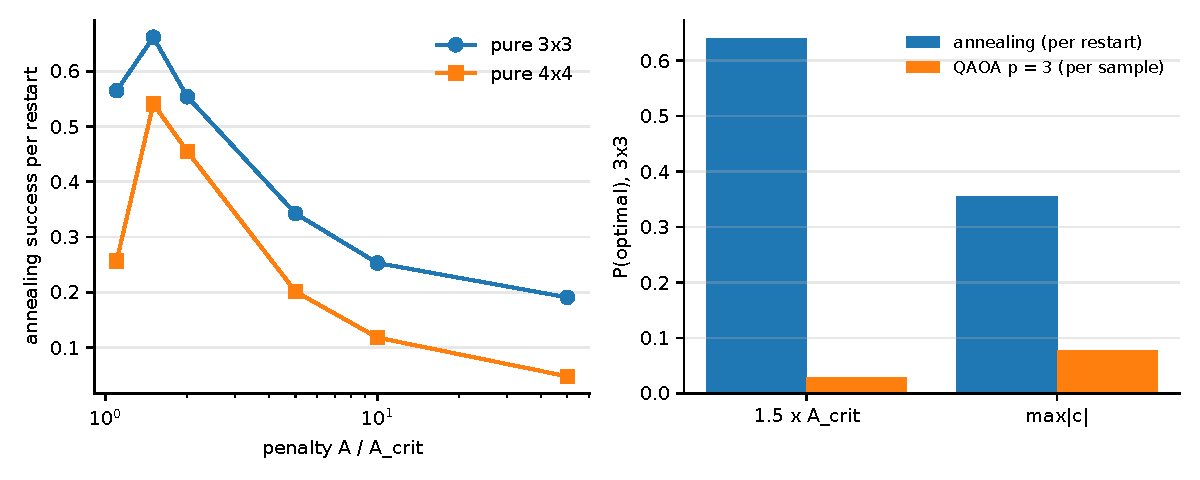
\includegraphics[width=\textwidth]{fig1_penalty.pdf}
\caption{Left: simulated-annealing success against the penalty relative to its exact critical value. Right: annealing and QAOA ($p=3$,
simulator) on the same $3\times3$ instances at two penalty rules.}\label{fig:penalty}
\end{figure}

\paragraph{QAOA.} The QUBO is mapped to an Ising Hamiltonian $H_C$ with $x_k = (1-Z_k)/2$. Starting from $\lvert+\rangle^{\otimes n}$, a
depth-$p$ circuit applies
\begin{equation}
\lvert\gamma,\beta\rangle = \prod_{l=1}^{p} e^{-i\beta_l\sum_k X_k}\, e^{-i\gamma_l H_C}\,\lvert+\rangle^{\otimes n},
\end{equation}
with the cost layer compiled to $R_Z$ and $R_{ZZ}$ rotations~\cite{farhi2014qaoa}. Angles were chosen by COBYLA minimising
$\langle\gamma,\beta\rvert H_C\lvert\gamma,\beta\rangle$ on an exact statevector simulator, from several random starts and, for $p>1$, a start
interpolated from depth $p-1$. The simulator was checked against Qiskit~\cite{javadi2024qiskit}. Two-qubit gate counts were estimated by
transpiling to a heavy-hex model and, for hardware runs, to the chosen device.

\paragraph{Hardware.} Circuits were run on \texttt{ibm\_kingston} with parameters from the simulator (Table~\ref{tab:p15}). The device was
chosen by the lowest median CZ error in that day's calibration data. Readout was corrected per qubit: calibration circuits preparing all
zeros and all ones give each measured qubit $q$ an assignment matrix $M_q$, and the measured distribution is multiplied by
$\bigotimes_q M_q^{-1}$, clipped at zero and renormalised. Of the four
predictions committed beforehand, three held and one held in part; the nine-qubit circuit, which an earlier step had expected to be
dominated by noise, kept most of its simulated value.

\begin{table}[h]
\centering
\begin{tabular}{lrrrr}
\toprule
circuit & CZ gates & $P(\mathrm{opt})$ simulator & hardware (corrected) & kept \\
\midrule
$2\times2$, $p=1$ & \PoneFiveTwoPoneCZ & \PoneFiveTwoPoneSim & \PoneFiveTwoPoneHw & \PoneFiveTwoPoneKept \\
$2\times2$, $p=2$ & \PoneFiveTwoPtwoCZ & \PoneFiveTwoPtwoSim & \PoneFiveTwoPtwoHw & \PoneFiveTwoPtwoKept \\
$3\times3$, $p=1$ & \PoneFiveThreePoneCZ & \PoneFiveThreePoneSim & \PoneFiveThreePoneHw & \PoneFiveThreePoneKept \\
\bottomrule
\end{tabular}
\caption{QAOA on \texttt{ibm\_kingston}: mean probability of the optimal string over 10 ($2\times2$) and 5 ($3\times3$) instances.}
\label{tab:p15}
\end{table}

\paragraph{Correction.} An intermediate penalty study reported an anomaly that turned out to be a fallback in the study code which left a
few instances without any penalty. It was found by the next step's independent check and corrected in the log.

\section{Multi-sensor assignment}\label{sec:p2}

\paragraph{Problem.} Three sensors at different positions observe the same targets at one instant; each reports positions with range and
bearing errors, misses targets and adds clutter. A hypothesis is a tuple $k=(i_1,i_2,i_3)$ of one measurement (or none, $i_s=0$) per sensor, with a
generalised likelihood-ratio cost~\cite{deb1997sd}. The target position is replaced by the weighted least-squares fusion
$\hat x_k = P_k\sum_{s\in D_k} R_s^{-1} z_s$ with $P_k = \bigl(\sum_{s\in D_k} R_s^{-1}\bigr)^{-1}$, where $D_k$ is the set of sensors
that saw it and $R_s$ each measurement's covariance, giving
\begin{equation}
c_k = \sum_{s\in D_k}\Bigl[-\ln P_D + \ln\lambda + \tfrac12 (z_s-\hat x_k)^\top R_s^{-1}(z_s-\hat x_k) + \tfrac12\ln|2\pi R_s|\Bigr]
      - \bigl(3-|D_k|\bigr)\ln(1-P_D).
\end{equation}
A single measurement may instead be declared clutter at cost zero. Valid associations are partitions of all measurements into tuples,
and the problem is the integer program
\begin{equation}
\min_{x\in\{0,1\}^K} \sum_k c_k x_k \quad\text{subject to}\quad \sum_{k\ni m} x_k = 1 \ \text{for every measurement } m.
\end{equation}
Its QUBO uses $Q_{kk} = c_k - A\,n_k$ and $Q_{kl} = 2A\,|k\cap l|$, where $n_k$ is the number of measurements in tuple $k$ and $|k\cap l|$
the number two tuples share. The pairwise gate rejected
\PtwoGateRejectedPct\,\% of \PtwoGateTruePairs{} true pairs, as expected for a 99\,\% chi-square gate.

\paragraph{Gates.} An integer program solved with HiGHS~\cite{huangfu2018highs,virtanen2020scipy} matched exhaustive partition
enumeration on all \PtwoILPGate{} instances checked, and the QUBO minimum matched the integer optimum on \PtwoQUBOGatePassed{} of
\PtwoQUBOGate{} brute-forceable instances; \PtwoQUBOInfeasible{} further scenes had no valid answer at all and were counted separately.

\paragraph{A failed hypothesis.} It was predicted that fusing three sensors would make the optimum equal the truth more often than in the
single-scan case. It did so in \PtwoHfourShare{} of three-target scenes (95\,\% Wilson interval \PtwoHfourLow--\PtwoHfourHigh~\cite{wilson1927}).
A one-factor study, labelled exploratory because it followed the result, traced this mainly to the cross-range error of bearing-limited
sensors (Figure~\ref{fig:truth}): the share rose from \PtwoFactorDefault{} to \PtwoFactorBearing{} when bearing error was reduced, and
to \PtwoFactorBearingNoClutter{} without clutter as well; with no clutter, no missed detections and no gate it was \PtwoFactorPure.
The prediction had compared unlike situations: single-scan association has track predictions as anchors, a snapshot does not.
Bearing error was then added to the benchmark sweep as a recorded amendment; the hypothesis stayed failed.

\begin{figure}[t]
\centering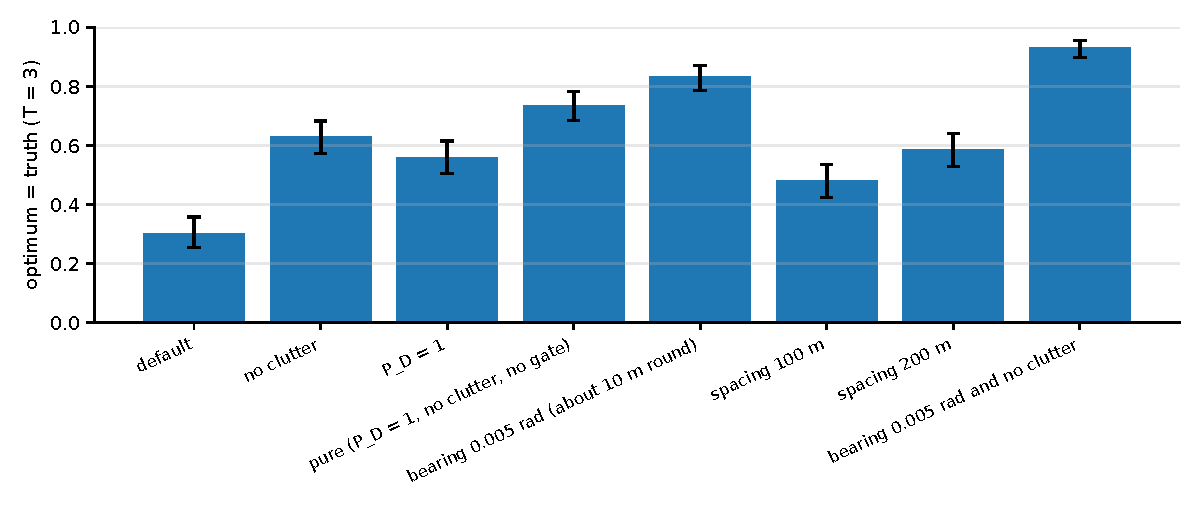
\includegraphics[width=\textwidth]{fig2_truth.pdf}
\caption{Share of three-target scenes in which the exact optimum equals the true association, changing one factor at a time
(exploratory; 95\,\% Wilson intervals).}\label{fig:truth}
\end{figure}

\paragraph{Classical baselines.} Greedy association takes tuples in order of cost and skips any that reuse a measurement. Simulated
annealing runs on the QUBO. Lagrangian relaxation moves the constraints of the third sensor into the objective with multipliers $u$,
\begin{equation}
L(u) = \sum_{j} u_j + \min_{x}\ \sum_k \bigl(c_k - u_{i_3(k)}\bigr)x_k \quad\text{subject to the sensor-1 and sensor-2 constraints},
\end{equation}
updates $u$ by subgradient steps, and recovers a feasible answer at each step with a second two-dimensional assignment. The inner problem
of $L(u)$ is a two-dimensional assignment problem whose solutions are integral, so the best Lagrangian bound equals the bound of the linear programming (LP) relaxation~\cite{geoffrion1974}, and the duality
gap could be measured exactly. Lagrangian relaxation reached the optimum in \PtwoLRLowClutter{} of scenes without clutter. The share of
scenes with a nonzero gap rose from \PtwoGapClutterZero{} to \PtwoGapClutterTwo{} with clutter, and from \PtwoGapSpacingFar{} to
\PtwoGapSpacingClose{} with closer spacing, but the intervals overlapped: the hypothesis was graded partly held. The first run of this
study crashed while saving its result file; after a one-line fix the rerun reproduced every printed number.

\paragraph{Benchmark.} The benchmark sweeps target count, clutter, detection probability, spacing and bearing error with three replicates:
\PtwoBenchInstances{} instances, each with its allowed tuples and costs, exact optimum, LP bound and true association, and a checker that
needs only the instance file. \PtwoBenchInfeasible{} instances have no valid answer; \PtwoBenchGap{} have an LP gap. A rebuild from the
recorded seeds reproduced every instance byte for byte. Table~\ref{tab:bench} and Figure~\ref{fig:bench} show the baselines scored by the
checker. Lagrangian relaxation stayed optimal on \PtwoBenchLRGap{} of the gap instances; its \PtwoBenchLRInvalid{} failures occur where its
recovery step cannot complete a pair (detection probability 1 with clutter), and greedy's \PtwoBenchGreedyInvalid{} where no
single-measurement tuple exists. The recovery step was later extended (see below).

\begin{table}[h]
\centering
\begin{tabular}{lr}
\toprule
method & share optimal \\
\midrule
Lagrangian relaxation, recovery as registered & \PtwoBenchLR \\
Lagrangian relaxation, recovery that may dissolve pairs (P2.8) & \PtwoEightLROptimal \\
simulated annealing (64 restarts, 100 sweeps) & \PtwoBenchSA \\
greedy & \PtwoBenchGreedy \\
greedy, per-measurement normalised & \PtwoBenchGreedyNorm \\
\bottomrule
\end{tabular}
\caption{Baselines on the solvable benchmark instances.}\label{tab:bench}
\end{table}

\begin{figure}[t]
\centering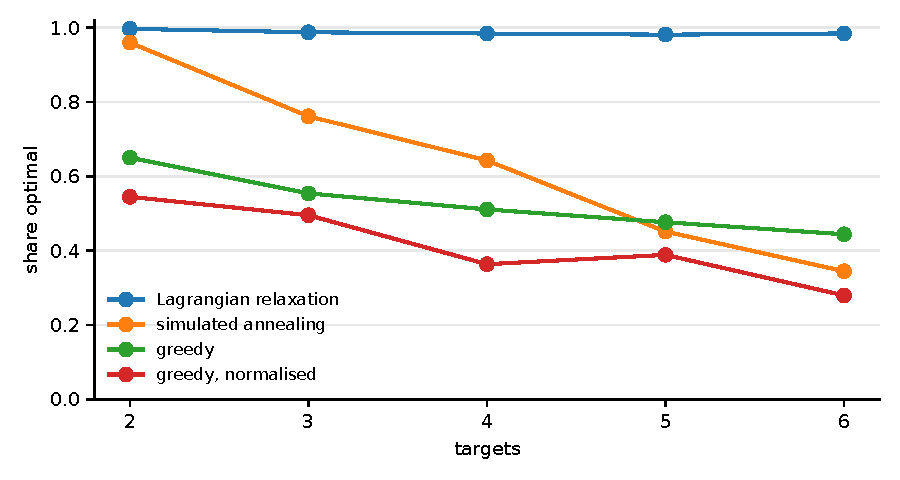
\includegraphics[width=0.75\textwidth]{fig3_baselines.pdf}
\caption{Share of benchmark instances solved optimally, by number of targets (recovery as registered).}\label{fig:bench}
\end{figure}

\paragraph{QAOA.} On eight-qubit instances QAOA again preferred the larger penalty: at $p=3$, \PtwoHthreeMaxAbs{} per sample with
$\max|c|$ against \PtwoHthreeOracle{} at $1.5\,A_\mathrm{crit}$, better on \PtwoHthreePurePositive{} of instances. On sparser instances
the mean pointed the same way but the larger penalty won on only \PtwoHthreeSparsePositive{} of instances; the penalty hypothesis was
graded partly held. The registered rule for spending hardware time --- at least five times the guessing probability with at most 60
two-qubit gates --- was met only by sparse instances at $p=1$ (\PtwoGoRatio{} times guessing, median \PtwoGoCZ{} CZ gates); the
eight-qubit instances were estimated to need \PtwoPureCZ{} CZ gates already at $p=1$ (transpiled to a generic heavy-hex model, not to a
specific device).

\paragraph{Hardware.} Two jobs were submitted after their predictions were public (Figure~\ref{fig:hw}). The P1 circuits rerun on a
second device, \texttt{ibm\_fez}, kept \PtwoSixAKept{} of the simulator value against \PoneFiveTwoPtwoKept{} on
\texttt{ibm\_kingston} --- the device half of a repeatability hypothesis; the run fell on the same calendar day, so the day half was
tested later (see below). Three-dimensional QAOA at $p=1$ on ten sparse instances (\PtwoSixBCZMin--\PtwoSixBCZMax{} CZ gates) reached
\PtwoSixBHw{} against \PtwoSixBSim{} on the simulator, \PtwoSixBGuess{} times guessing. Two of five numeric predictions missed, both by
less than the shot noise. The jobs used \PtwoSixUsage{} seconds of processor time.

\begin{figure}[t]
\centering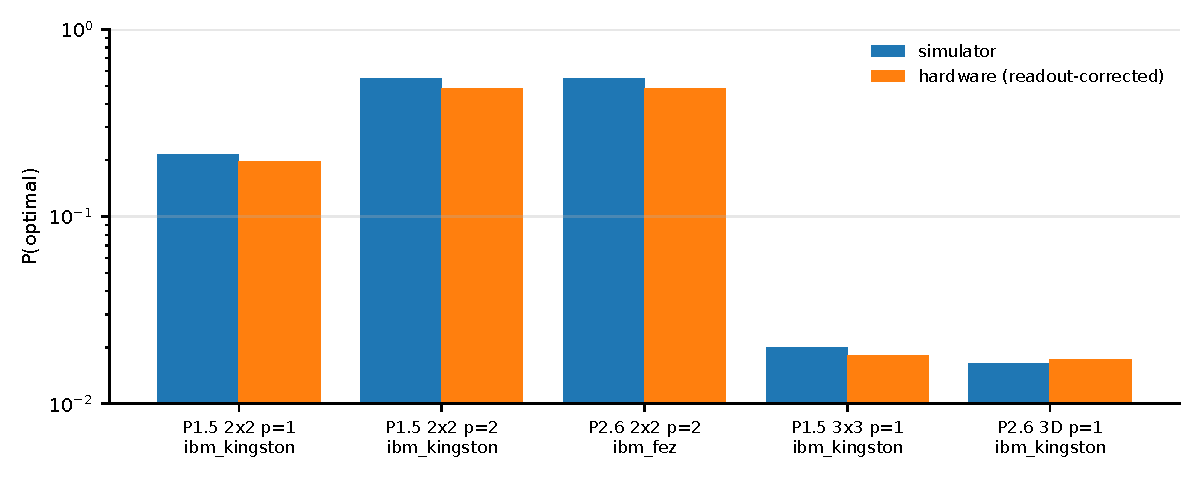
\includegraphics[width=\textwidth]{fig4_hardware.pdf}
\caption{Simulator and readout-corrected hardware probability of the optimal string for the P1 and P2 hardware QAOA runs.}\label{fig:hw}
\end{figure}

\paragraph{Closing the open items (P2.8).} The P2 summary left four questions open. After the report's first version they were given
hypotheses in a second amendment and run (Table~\ref{tab:hypotheses}).
\begin{enumerate}
\item \emph{Another day.} The P1 circuits on \texttt{ibm\_kingston} one day later kept \PtwoEightHfiveKept{} after readout correction:
      held. Without correction they kept only \PtwoEightHfiveRawKept, because one physical qubit read 0 as 1 in \PtwoEightBadQubit{} of the
      job's own calibration shots, although the device's calibration data from that morning reported a normal readout error for it.
\item \emph{Recovery.} Allowing the recovery step to dissolve a relaxed pair into two single-measurement tuples made Lagrangian
      relaxation return a valid answer on \PtwoEightLRValid{} of solvable instances and the optimum on \PtwoEightLROptimal; all
      \PtwoEightLRFormerFailures{} former failures became optimal and no instance lost its optimum: held.
\item \emph{Marginal likelihood.} Integrating the target position out under a uniform prior over the scene window of area $V$,
      instead of fitting it, changes the cost to
      \begin{equation}
      c_k^{\mathrm{marg}} = c_k + \ln V - \tfrac12\ln\left|2\pi P_k\right| .
      \end{equation}
      On the benchmark this joined \PtwoEightJoinedMarginal{} of \PtwoEightClutterMeasurements{} clutter measurements into
      multi-measurement tuples instead of \PtwoEightJoinedGLR{} (fewer in \PtwoEightJoinedBetter{} instances, more in
      \PtwoEightJoinedWorse), but the optimum equalled the truth as often as before (\PtwoEightTruthGain{} instances gained,
      \PtwoEightTruthLoss{} lost): partly held.
\item \emph{Objective.} Training QAOA on the mean energy of the lowest-energy tenth of the output distribution
      (CVaR~\cite{barkoutsos2020cvar}) instead of the full expectation raised the probability of the optimum on the sparse instances at
      $p=1$ from \PtwoEightExpPone{} to \PtwoEightCvarPone, but lowered it at $p=3$ from \PtwoEightExpPthree{} to \PtwoEightCvarPthree:
      partly held.
\end{enumerate}
The hardware job used \PtwoEightUsage{} seconds of processor time.

\section{Reproducing a published result}\label{sec:p3}

\paragraph{Target.} QANTIS~\cite{eker2026qantis} reports QAOA with a fixed number of schedule parameters~\cite{saavedra2025fpc} on a
two-track, three-measurement instance (11 qubits) on IBM hardware, with a headline solution quality of
\PthreePaperHeadline\,\% $\pm$ \PthreePaperHeadlineSD\,\% of the optimum at $p=3$ using \PthreePaperTwoQubitGates{} two-qubit gates. It was the only
gate-model data-association result with hardware data and public code found by the literature searches for this study. A plan registered four of its claims and four
added questions before any code; a source audit of the paper and its public repository preceded the experiments. Only the public code
was available.

\paragraph{Instances.} An independent re-implementation produced QUBO matrices identical to those of the authors' code for both
hardware instances. The optimum of the small instance is $\PthreeOptimum$, against the paper's $\PthreePaperHungarian$ (difference
\PthreeCOneDiff); the larger instance gives $\PthreeOptimumLarge$ against $\PthreeLargePaperOptimum$. These values require a clutter-density
term that the code adds to every cost but the paper's cost equation omits; with the equation as printed the small instance has optimum
$\PthreeOptimumPaperEq$ and a different optimal association.

\paragraph{Method.} Implemented from the paper and simulated without noise, the method reached a mean quality of \PthreeQualityA{} at $p=3$,
above the reported hardware value, so the simulated claim was reproduced. Its probability of the optimal string was \PthreePoptA.

\paragraph{The metric.} For a sample of 4096 shots, let $T_{10}$ be the ten most frequent bitstrings. The paper's quality is
\begin{equation}
q = \frac{\min_{x\in T_{10}} x^\top Q\, x}{E^\star},
\end{equation}
with $E^\star<0$ the optimal QUBO value, so $q=1$ when the optimum is among the ten. Uniformly random bitstrings give a mean of \PthreeRandomMean{} with a 95th percentile of \PthreeRandomPninetyfive, and reach the
headline value in \PthreeRandomAboveHeadline{} of samples (Figure~\ref{fig:metric}). By the rule registered before the result, the headline
does not distinguish a working circuit from random sampling. The best of all samples, the measure behind the paper's simulator values, is
weaker still: random sampling scores \PthreeRandomBestOfAll. On the 19-variable instance the noiseless method reached \PthreeLargeQualityPone{}
($p=1$) and \PthreeLargeQualityPtwo{} ($p=2$), while random sampling averaged \PthreeLargeRandomMean{} and reached the reported hardware
value of \PthreeLargePaperPone{} in \PthreeLargeRandomAbove{} of samples; the reported $p=2$ value, \PthreeLargePaperPtwo, is below the random
mean.

\begin{figure}[t]
\centering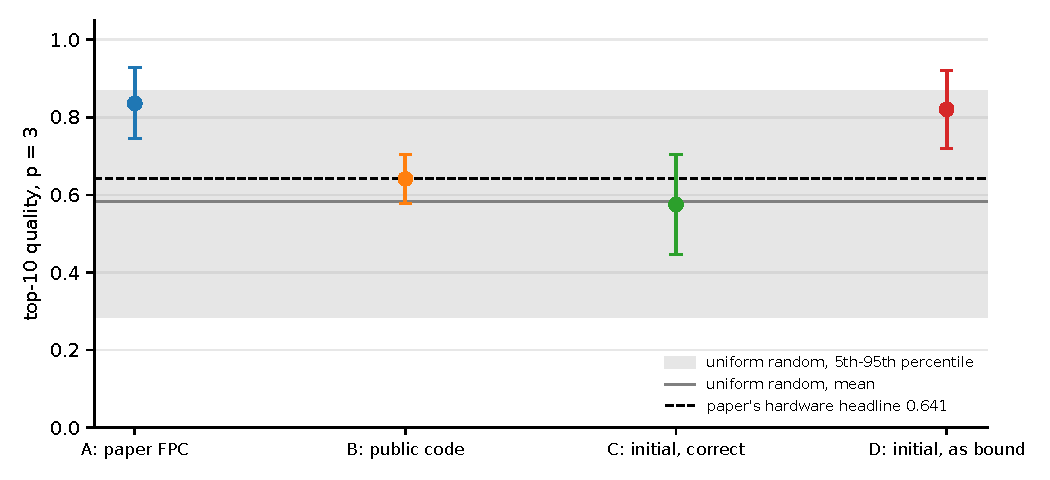
\includegraphics[width=0.85\textwidth]{fig5_metric.pdf}
\caption{The paper's quality metric at $p=3$ for four circuit variants (mean and standard deviation over 200 samples of 4096 shots)
against uniformly random bitstrings. A: method as described; B: public solver; C: analytical initial schedule; D: the same schedule as
bound by the public hardware script.}\label{fig:metric}
\end{figure}

\paragraph{Code defects.} Three defects were confirmed in the public code with the authors' toolchain. (1)~On the initial-schedule path
the hardware script binds an interleaved list of angles to parameters that Qiskit orders with all $\beta$ before all $\gamma$; on the
metric the misbound circuit scored \PthreeQualityD{} and the correctly bound one \PthreeQualityC. (2)~Bitstrings are evaluated in mirror
order: the variable-to-qubit mapping is the identity, but count keys are read left to right, which would lower the noiseless $p=3$ score
from \PthreeQualityA{} to \PthreeReversedA{} without changing the quantum state. (3)~The public solver trains all $2p$ angles and uses the
schedule only as a starting point, so it does not implement a fixed number of parameters. Whether the authors' private code shares these
defects is unknown.

\paragraph{Not tested.} The hardware claim was not rerun: since its registered metric cannot separate signal from noise, a rerun could
not confirm or refute it. The findings were sent by email to the correspondence address given in the paper on 15~September~2026,
before the first version of this report was archived. Archiving was not held back for a reply; any response will be recorded in the
repository, and a corrected version will be issued if one is needed.

\section{Constraint-preserving mixers}\label{sec:p5}

\paragraph{Question.} Every QAOA circuit above enforced the assignment constraints with a penalty, and most of its samples were not valid
associations. The quantum alternating operator ansatz instead uses a mixer that never leaves the set of valid
answers~\cite{hadfield2019qaoa,wang2020xy,fuchs2022constraint}. On the 50 pure $3\times3$ instances of P1, three ans\"atze were compared
at equal depth and with the same optimiser:
\begin{itemize}
\item \emph{penalty} --- the P1 circuits, with the $X$ mixer and the penalty $A=\max|c|$;
\item \emph{row XY} --- a W state on each row, rotations $e^{-i\beta(\lvert01\rangle\langle10\rvert + \lvert10\rangle\langle01\rvert)}$ on every pair of
      qubits within a row, and a penalty on the columns only;
\item \emph{permutation} --- a uniform superposition of the $3!$ permutations, rotations between $\lvert1100\rangle$ and $\lvert0011\rangle$ on
      the four cells shared by two rows and two columns, and no penalty.
\end{itemize}
Transpiled circuits matched the simulator to $\PfiveGateMaxDiff$, and no probability left the preserved space.

\begin{table}[h]
\centering
\begin{tabular}{lrrrr}
\toprule
ansatz & $P(\mathrm{opt})$, $p=1$ & $P(\mathrm{opt})$, $p=3$ & gain over own space, $p=1$ & CZ, $p=1$ \\
\midrule
penalty & \PfiveXpenPone & \PfiveXpenPthree & \PfiveXpenLiftPone & \PfiveXpenCZ \\
row XY & \PfiveRxyPone & \PfiveRxyPthree & \PfiveRxyLiftPone & \PfiveRxyCZ \\
permutation & \PfivePermPone & \PfivePermPthree & \PfivePermLiftPone & \PfivePermCZ \\
\bottomrule
\end{tabular}
\caption{Pure $3\times3$ instances, mean over 50. Gate counts: heavy-hex model, generic state preparation, median of 5 instances.}\label{tab:p5}
\end{table}

\paragraph{Result.} Each restriction raised the probability of the optimum at every depth (H1, H2 held; Table~\ref{tab:p5}). Part of this is
only the smaller search space --- uniform guessing finds the unique optimum with probability $1/512$, $1/27$ and $1/6$ in the three spaces ---
and measured against its own space the penalty circuit gains most at $p=1$; the permutation circuit still improved on its starting state
by a factor of \PfivePermLift{} $\pm$ \PfivePermLiftSE{} at $p=3$ (H3 held). No constraint-preserving circuit fitted the hardware budget of
60 two-qubit gates (H4 failed), so no hardware time was used.

\section{Reproducing the planning results}\label{sec:p6}

\paragraph{Target.} The second half of QANTIS~\cite{eker2026qantis} applies quantum belief updates to the Tiger
problem~\cite{kaelbling1998planning}: two states, listening correct with probability \PsixPaperListen{} and discount \PsixPaperGamma. (It
is unrelated to quantum POMDPs in the sense of~\cite{barry2014qpomdp}.) A belief oracle prepares
\begin{equation}
A\lvert00\rangle = \sum_{s,o}\sqrt{b(s)\,O(o\mid s)}\;\lvert s,o\rangle ,
\end{equation}
so that post-selecting the observation $o$ leaves the Bayesian posterior $b'(s)\propto b(s)\,O(o\mid s)$. One Grover
iterate~\cite{grover1996,brassard2002amplitude} with the reflections $S_o$ (on the observation) and $S_0$ (about $\lvert00\rangle$) raises the
probability of a rare observation from $\sin^2\theta$ to
\begin{equation}
P\bigl(o \mid A S_0 A^\dagger S_o A\lvert00\rangle\bigr) = \sin^2 3\theta ,
\end{equation}
without changing the post-selected posterior. Actions are chosen classically by a planner that looks one step ahead. A plan registered
seven claims and three questions, and a source audit read the paper and the public code at the commit dated with the paper.

\paragraph{Simulator claims.} With circuits rebuilt from the paper, one iterate gave \PsixCOneBase{} $\to$ \PsixCOneGrover{} with posterior
\PsixCOnePostLeft{} for the likely state, matching the stated \PsixPaperTheoryBase{} $\to$ \PsixPaperTheoryGrover{} (C1 reproduced); all belief
circuits gave exact posteriors, within $\PsixCTwoMax$ in Hellinger distance (C2), and the closed loops chose the reported actions (C4). Two
statements did not hold. The paper's table of amplified probabilities gives \PsixPaperTableOne{} and \PsixPaperTableThree{} after one and three
iterates where $\sin^2(2G{+}1)\theta$ gives \PsixCSixFormulaOne{} and \PsixCSixFormulaThree, and its section formula for the number of
iterates gives \PsixCSixSectionIterations{} where the table states \PsixPaperTableIterations{} (C6). A Hellinger threshold of \PsixPaperPass{}
is said to mean at most \PsixPaperTV\,\% total-variation distance, but total variation lies between $H^2$ and $H\sqrt{2-H^2}$; the
distributions $(\tfrac12,\tfrac12)$ and one at Hellinger distance \PsixCSevenH{} from it already differ by \PsixCSevenTV{} (C7).

\paragraph{Circuit sizes.} The paper defines its ``ISA depth'' as the two-qubit gate count after transpilation. Transpiling the public circuits
to an offline Heron model gave \PsixCThreeListenCZ{} and \PsixCThreeGroverCZ{} two-qubit gates but total depths of \PsixCThreeListenDepth{}
and \PsixCThreeGroverDepth{} --- the reported \PsixPaperISAListen{} and \PsixPaperISAGrover{} are total depths. The four-state circuit
(\PsixCThreeFourCZ{} gates, depth \PsixCThreeFourDepth, reported \PsixPaperISAFour) and the full eleven-qubit circuit (\PsixCThreeFullCZMin--\PsixCThreeFullCZMax{}
gates, depth \PsixCThreeFullDepthMin--\PsixCThreeFullDepthMax, reported \PsixPaperISAFull) matched neither count (C3 not reproduced).

\paragraph{Hardware.} The only claim small enough to test was run once, in three replicates on \texttt{ibm\_kingston}, after five numeric
predictions were public. The probability of the rare observation rose from \PsixHwBase{} to \PsixHwGrover, an amplification of \PsixHwAmp,
with a posterior Hellinger distance of \PsixHwHellinger{}, against the reported \PsixPaperBase{} $\to$ \PsixPaperGrover{} and
\PsixPaperAmp-fold: reproduced, with all five predictions held, using \PsixHwUsage{} seconds of processor time.

\paragraph{Counting the gain.} The amplified circuit applies the belief oracle three times per shot --- $A$, $A^\dagger$ and $A$ again ---
while the direct circuit applies it once. Per application of the oracle, the quantity that the paper's $O(P(e)^{-1/2})$ argument
concerns, the gain in usable samples is \PsixQOneTheory-fold in theory and \PsixHwPerOracle-fold on hardware, not the
\PsixPaperAmp-fold counted per shot.

\paragraph{Planning table.} The public simulation entry point reports only an average reward of $\PsixCFiveEntryReward$ per episode: its
belief never changes and the configured baseline planners are never called. The paper does not state the rewards, whether they are
discounted or what follows a door being opened, so the table could not be rebuilt (C5 not reproducible). An exact solution by value
iteration gives $V^\star(\tfrac12)=\PsixQTwoValue$ and opens a door below a posterior of \PsixQTwoThreshold{} where the one-step planner opens
below \PsixQTwoGreedyThreshold; plausible protocols gave rewards of \PsixCFiveHorizonMean{} $\pm$ \PsixCFiveHorizonSD{} and
\PsixCFiveOptimalMean{} $\pm$ \PsixCFiveOptimalSD{} against the table's \PsixPaperTableSixQBRL{} $\pm$ \PsixPaperTableSixSD{} (exploratory).

\paragraph{Paper and code.} The public scripts pass a result at a Hellinger distance below \PsixCodePass, not \PsixPaperPass; under the code's
threshold the reported four-state result of \PsixPaperFourObsZero{} would fail. The four-state circuit applies the same gates for either
observation, although the paper explains the difference between the two by different gate paths. Two references in the paper name the
wrong authors.
The findings of this section were sent by email to the correspondence address given in the paper on 15~September~2026, before this
version of the report was archived; any response will be recorded in the repository, and a corrected version will be issued if one
is needed.

\section{Lessons across the project}

\begin{enumerate}
\item \emph{Penalty weights are solver-specific.} Annealing preferred penalties just above the critical value; QAOA preferred larger ones,
      in both two- and three-dimensional problems.
\item \emph{The optimum is not the truth.} Model and sensor limits bounded accuracy long before solvers did; solver comparisons must be
      made against the optimum. A better-founded cost removed spurious clutter associations without improving that accuracy.
\item \emph{A metric needs a random baseline.} ``Best of $k$ samples'' can be high for noise; the probability of the optimal or of a
      feasible string, compared with uniform sampling over the same space, carries the evidence.
\item \emph{Count a speed-up in the resource the argument is about.} A gain per circuit run can be three times the gain per oracle call.
\item \emph{Constraints can be kept, at a price.} Constraint-preserving mixers raised the probability of the optimum by an order of magnitude
      but needed more two-qubit gates than current hardware budgets allow.
\item \emph{Shallow circuits transferred well; calibration must be measured.} On two Heron devices, circuits with up to about 60 two-qubit
      gates kept roughly nine tenths of their simulated success probability where that probability was well above guessing, and a
      published two-qubit hardware result repeated closely. On one day a qubit misread almost every zero although the device reported it as
      normal; only calibration inside the job caught it.
\item \emph{Independent checks find bugs.} Gates and cross-checks exposed a bug in this project's own study code, three defects in a
      published artefact and, in its planning half, numbers that did not match their definitions; predictions committed before results kept
      failed hypotheses visible.
\end{enumerate}

\section{Limits}

Instances are small and synthetic, generated from one model per phase. Hardware runs used one calibration window per job and ten or fewer
instances per setting. The first reproduction used only public code, a noiseless simulator and one instance per size, as in the paper; the
second re-ran one hardware experiment, the smallest, on a different device from the paper's, and measured circuit sizes on an offline
backend model. The constraint-preserving mixers were not run on hardware. No result here bears on quantum advantage. The project used
\QPUSecondsTotal{} seconds of quantum processor time in total.

\section*{Data and code availability}
All code, data, plans, results and corrections are at \url{https://github.com/kbksqa/quantum-lab}; every release is archived on Zenodo
under the concept DOI \href{https://doi.org/10.5281/zenodo.22741037}{10.5281/zenodo.22741037}. All data are synthetic or public.

\section*{AI-assistance disclosure}
Code, analysis and drafting were carried out with the assistance of an AI system (Claude, Anthropic). The author directed
the work, reviewed every result and takes full responsibility for the content.

\appendix
\section{Grover search and readout error}
Before the optimisation studies, Grover search~\cite{grover1996} on three qubits was run on \texttt{ibm\_kingston} to calibrate expectations.
At two iterations the success probability was \PzeroKingstonHardware{} against \PzeroKingstonTheory{} in theory. Readout calibration on three
devices recovered only \PzeroFiveGainMinPP--\PzeroFiveGainMaxPP{} percentage points (on \texttt{ibm\_kingston} from \PzeroFiveKingstonRaw{}
to \PzeroFiveKingstonCorrected), so most of the loss came from gates rather than measurement.

\section{Benchmark format}
Each instance is one JSON object holding the generator seed and parameters, sensor positions, measurements and covariances, the true
association, every allowed tuple with its cost, the exact optimum and its partition, and the LP bound. A valid answer is a set of allowed
tuples that uses every measurement exactly once; the checker reports validity, cost, gap to the optimum and agreement with the truth using
only the Python standard library. The format is documented in \texttt{benchmark/p2/README.md}.

\bibliographystyle{unsrt}
\bibliography{refs}

\end{document}
